\section{Related Work}
\label{sec:related}

\begin{figure*}[t]
  \centering
  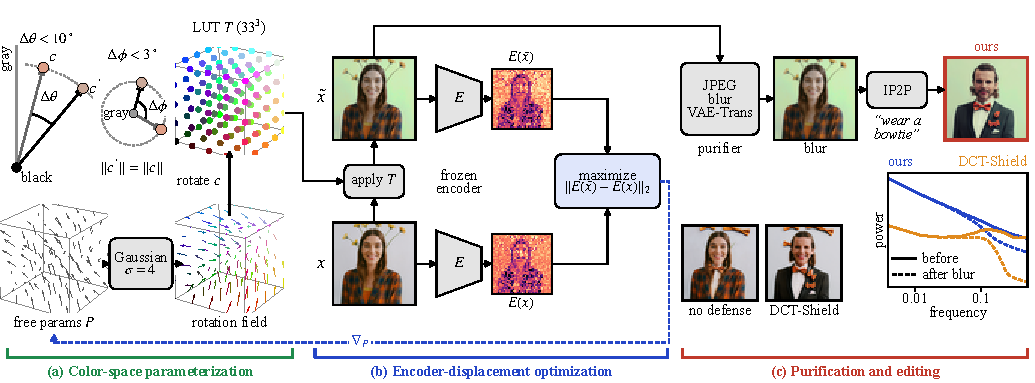
\includegraphics[width=\linewidth]{fig/method_overview.pdf}
  \caption{Overview of color-mapping immunization. (a)~Free parameters $P$ on a $33^3$ grid are smoothed by a Gaussian kernel ($\sigma = 4$ grid cells) into a rotation field. The field rotates each color vector $c$ about the black point and preserves $\|c\|$. With the gray axis as the polar axis, the polar angle changes by less than $10^\circ$ and the azimuth by less than $3^\circ$ before clipping to the RGB gamut; the angles in the sketch are enlarged. (b)~The resulting LUT $T$ is applied to the image $x$, and $P$ is optimized to maximize the displacement $\|E(\tilde{x}) - E(x)\|_2$ of the frozen VAE encoder $E$. (c)~The attacker purifies the protected image $\tilde{x}$ (here Gaussian blur, $\sigma = 2$) and edits it with InstructPix2Pix (``Let the person wear a bowtie''). The edit of our protected image replaces the person; after the same blur, the DCT-Shield~\cite{dctshield2025} protection keeps the person and changes only the clothing. ``No defense'' is the edit of the unprotected original. The spectra show the perturbation power averaged over eight portraits before (solid) and after (dashed) blur, each on its own unlabeled vertical scale.}
  \label{fig:overview}
\end{figure*}

\paragraph{Immunization against diffusion editing.}
PhotoGuard~\cite{salman2023photoguard} introduced protection against Stable Diffusion editing with an encoder attack and a costlier diffusion attack. Later methods kept the additive form and changed the target or the budget. Mist and AdvDM~\cite{liang2023mist,liang2023advdm} combine a textural loss on the encoder with a semantic loss on the denoiser. EditShield~\cite{chen2024editshield} targets instruction-guided editing, DIA~\cite{dia2025} attacks the inversion trajectory of inpainting, FaceLock~\cite{wang2025facelock} protects facial identity, and DiffVax~\cite{diffvax2026} replaces per-image optimization with a trained feed-forward network. \TODO{SIFM, DANP, DAYN.} Protections for DiT editors~\cite{decontext2025,nulledit2026} also use additive perturbations. Robustness-oriented variants change where the perturbation is placed. DCT-Shield~\cite{dctshield2025} perturbs JPEG coefficients, DiffusionGuard~\cite{diffusionguard2025} targets the early denoising steps, and BlurGuard~\cite{blurguard2025} applies region-wise blur to the noise. In every case the protection remains an additive pattern on the pixel grid, which is the component that blurring, compression, and reconstruction attenuate. We keep the threat model of this line of work and replace the carrier.

\paragraph{Purification.}
Simple operations remove protective perturbations. JPEG compression~\cite{sandoval2023jpeg} and noisy upscaling~\cite{honig2025noisyupscaling} bypass several protections, and H\"{o}nig~\etal~\cite{honig2025noisyupscaling} argue that the defender is structurally disadvantaged because the protection must be fixed before the attacker chooses a purification. VAE-based purifiers remove the protection of six methods without knowledge of how the images were protected~\cite{purifyonce2026}, and CAT~\cite{cat2025} removes it by fine-tuning a small adapter. Other studies find that edits of protected images often still follow the prompt~\cite{icip2025disruptive} and that protections fail under chains of common transformations~\cite{doprotect2026}. These works establish that additive protections can be removed, and they evaluate each protection at its own budget. We adopt the image-space purifications of this literature as part of the evaluation and compare all defenses at matched distortion.

\paragraph{Color-based adversarial examples.}
Adversarial examples for image classifiers need not be additive noise. Hue and saturation shifts~\cite{hosseini2018semantic}, per-image color lookup tables~\cite{laidlaw2019functional}, piecewise-linear color filters~\cite{zhao2020ace,zhao2023advcf}, and semantic recoloring~\cite{shamsabadi2020colorfool,bhattad2020cadv} all cause misclassification. Natural Color Fool~\cite{yuan2022ncf} restricts colors to distributions observed in real images, and AdvCF~\cite{zhao2023advcf} found color filters more robust than noise to JPEG and filtering. These attacks target classifiers and bound the color change with $\ell_p$ radii on the table or with semantic color ranges, which assume a classification decision as the outcome. We take the per-image lookup table of ReColorAdv~\cite{laidlaw2019functional} as the carrier, apply it to immunization against diffusion editing, and bound it with a smooth rotation of saturation and hue (\cref{sec:feasible}).

\paragraph{Judging color changes.}
LPIPS and DISTS~\cite{zhang2018lpips,ding2020dists} compare deep features of an image and its reference, and CIEDE2000~\cite{sharma2005ciede2000} compares colors pixel by pixel. S-CIELAB~\cite{zhang1997scielab} adds spatial filtering that models color acuity, CD-Flow~\cite{chen2023cdflow} learns a color difference for photographs, and the measure of Rajashekar~\etal~\cite{rajashekar2010color} tolerates changes of illumination. Preference models~\cite{kirstain2023pickscore,ma2025hpsv3} score an image against a text prompt, and SCOOTER~\cite{scooter2025} provides a protocol for human studies of unrestricted adversarial examples. Reference-based measures, including PSNR and SSIM, count a global change of tone as error and therefore rank a color-graded image below additive noise of equal LPIPS. We report LPIPS as the common distortion axis, add no-reference aesthetic scores, and follow the principle of~\cite{rajashekar2010color} with a color-aligned distortion that factors out the best-fitting global color transform before comparison.
